\chapter{Сравнение с существующими решениями}

Разработанный алгоритм сложно сравнивать с другими из-за специфики исходных данных. 
Средняя длина сообщений примерно равна 30 символам, а распределение по длинам показано на рис.~\ref{fig10}.

\begin{figure}[h!]
  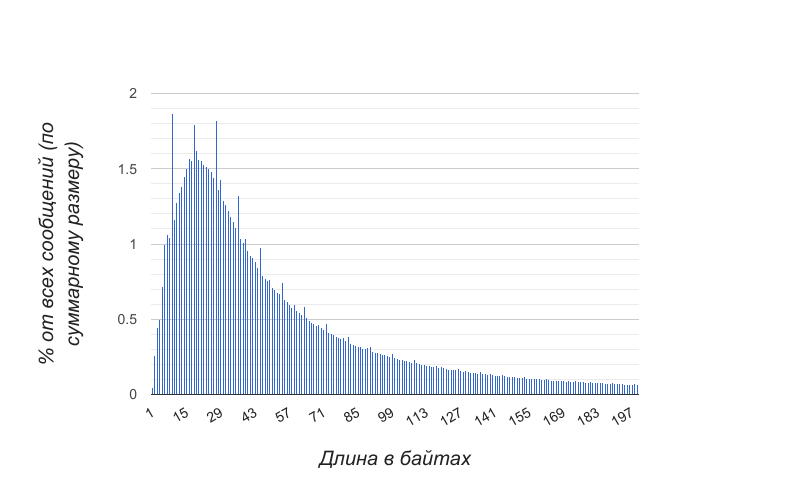
\includegraphics[width=\linewidth]{pics/msgs-len.png}
  \caption{Распределение сообщений по их длинам}
  \label{fig10}
\end{figure}

Проблема заключается в том, что большинство алгоритмов сжатия рассчитаны на сжатие большого объема данных.
В случае же когда сообщения имеют длину порядка 30 байт, то такое сообщение, чаще всего, при сжатии стандартными архиваторами,
станет еще больше. Конечно, можно сжимать сразу весь набор сообщений, но тогда сравнение будет некорректным, так как 
такой метод не позволяет получить произвольное сообщение быстро, а значит решение противоречит поставленной задаче.

Поэтому для сравнения можно брать известные алгоритмы и пытаться модифицировать их так, чтобы они стали применимы к исходной задаче, либо
использовать алгоритмы, которые дают возможность обучиться на некотором наборе данных, а потом использовать полученный словарь, чтобы 
сжимать новые данные.

\section{LZW}
Алгоритм Лемпеля-Зива-Велча (LZW) был опубликован в 1984 году \cite{lzw}.
Идея алгоритма заключается в следующем. Создадим таблицу из слов размера $2^k$ для некоторого $k$. Изначально в нее поместим только отдельные буквы.
Данная таблица будет пополняться по мере кодирования сообщений. Так при кодировании находится наибольшее слово, которое уже есть в словаре, 
записывается позиция этого слова в таблице, а также в таблицу добавляется слово на один большей длины. Значение $k$ при этом может динамически увеличиваться.

Этот алгоритм необходимо было несколько адаптировать под рассматриваемую задачу. А именно, поскольку сообщения короткие, предлагается вначале 
<<прогнать>> алгоритм через все сообщения, чтобы набрать базу слов, а потом кодировать отдельные сообщения с использованием полученной таблицы.
При этом необходимо побороться с тем, что таблица может переполниться. Чтобы такого не произошло будем удалять самые старые слова для освобождения места.

При этом необходимо следить, чтобы не было ситуации, когда некоторое слово есть в таблице, а его префикса нет. Такая ситуация приводит к бесполезной трате оперативной памяти.
Чтобы такого не случалось, необходимо при использовании некоторого слова, переместить все его префиксы в начале LRU (двусвязного списка для удаления старых слов).

Кроме того непонятно, какое значение $k$ использовать. Очевидно, что для маленького количества сообщений необходимо использовать $k$ поменьше, а для большого~--- больше. 
Чтобы определить оптимальное значение было проведено несколько экспериментов с разными $k$.

На рис.~\ref{fig11} показано сравнение разработанного алгоритма и алгоритмов LZW с различными значениями $k$. В качестве набора сообщений для тестов был взят тот же набор,
что описывался в главе про разработку алгоритма.

\begin{figure}[h!]
  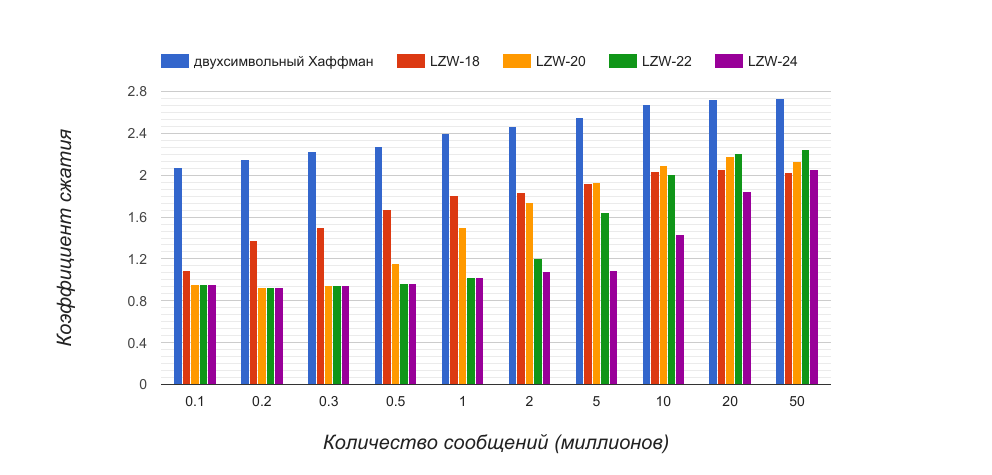
\includegraphics[width=\linewidth]{pics/lzw.png}
  \caption{Сравнение разработанного алгоритма с LZW}
  \label{fig11}
\end{figure}

Как видно из рисунка, разработанный алгоритм достаточно сильно выигрывает у LZW вне зависимости от $k$. Что же касается выбора размера таблицы, то видно,
что на наборах с 20 и 50 миллионами сообщений выигрывает таблица размером $2^{22}$, на 5 и 10 миллионах лучший размер~--- $2^{20}$, а на всех остальных тестах лучше всего
показал себя алгоритм с маленькой таблицей.

\section{SMAZ}

SMAZ~--- одна из немногих библиотек, которые рассчитаны на сжатие коротких текстов \cite{smaz}. В частности, в описании проекта
упоминается, что большинство алгоритмов не могут сжать сообщения длиной меньше 100 символов, а SMAZ может сжать слово \text{the} до одного байта.

Внутри у данного алгоритма фиксированный набор самых часто употребляемых английских слов. Поэтому, если сжимается английский текст, то он может достигнуть 
коэффициента сжатия порядка двух (это все еще значительно меньше чем разработанный нами алгоритм), а на русскоязычных текстах SMAZ не может ничего сжать.

Поскольку smaz рассчитан только на сжатие английских текстов, для сравнения была создана отдельная выборка сообщений. В нее были включены
только сообщения без кириллических символов. Всего было использовано пять миллионов сообщений. Однако, оказалось, что smaz не может сжать эти данные хорошо.
А именно, суммарный размер сообщений после сжатия оказался примерно равным исходному размеру сообщений. 

Такой плохой результат объясняется спецификой сжимаемых данных. Большинство сообщений из набора~--- ссылки и смайлики. А smaz внутри себя содержит 
набор наиболее встречающихся английских слов, которые в данном наборе встречались довольно редко. 

Результаты некоторых других алгоритмов, которые были рассмотрены в работе, показаны в таблице~\ref{tab1}.

\begin{table}[!h]
\caption{Коэффициенты сжатия для сообщений без кириллических символов}\label{tab1}
\centering
\begin{tabular}{|*{2}{c|}}\hline
Алгоритм & Коэффициент сжатия \\\hline
SMAZ & 1,020 \\\hline
Односимвольный Хаффман & 1,389 \\\hline
Хаффман по словам & 1,854 \\\hline
LZW & 2,022 \\\hline
Хаффман по словам + односимвольный Хаффман & 2,282 \\\hline
Хаффман по словам + двухсимвольный Хаффман & 2,391 \\\hline
\end{tabular}
\end{table}

Поскольку на сообщениях пользователей <<В Контакте>> алгоритм smaz показал себя очень плохо, было проведено сравнения алгоритма на обычном английском тексте.
Для этого были использованы тексты книг на английском языке из проекта <<Гутенберг>>~\cite{gutenberg}. Сам текст был разбит на сообщения длиной порядка 40 символов.
Суммарный размер сообщений 6,5 мегабайт, а всего их было 150 тысяч. На таких данных smaz смог достигнуть коэффициента сжатия 1,728, что уже достаточно хорошо,
но все равно уступает разработанному алгоритму. Сравнение алгоритмов представлено в таблице~\ref{tab2}. Заметим, что двухсимвольный Хаффман
показал себя хуже чем односимвольный, так как суммарный размер сообщений слишком маленький.

\begin{table}[!h]
\caption{Коэффициенты сжатия для проекта Гутенберг}\label{tab2}
\centering
\begin{tabular}{|*{2}{c|}}\hline
Алгоритм & Коэффициент сжатия \\\hline
Односимвольный Хаффман & 1,726 \\\hline
SMAZ & 1,728 \\\hline
LZW & 1,957 \\\hline
Хаффман по словам & 2,614 \\\hline
Хаффман по словам + двухсимвольный Хаффман & 2,676 \\\hline
Хаффман по словам + односимвольный Хаффман & 2,936 \\\hline
\end{tabular}
\end{table}


\section{zstd}

Довольно интересным является алгоритм zstd, предложенный Facebook \cite{facebook}. Кроме того,
что он имеет хороший коэффициент сжатия и скорость, он также имеет возможность обучаться на выборке сообщений.

В описании алгоритма есть целый раздел про дополнительное обучение алгоритма, в котором сказано, что оно помогает существенно улучшить степень сжатия JSON размером порядка килобайта.

Сравнение алгоритмов проводилось на выборке из пяти миллионов сообщений, суммарный размер которых 128 мегабайт. Для тренировки алгоритма zstd все сообщений необходимо сохранить в виде отдельных файлов, а потом передать их в качестве аргументов запуска. Из-за ограничения на количество передаваемых аргументов и скорости работы операционной системы с большим количеством маленьких файлов, было 
решено соединить сообщения в группы и сжимать целыми группами.

В качестве первого эксперимента сообщения были собраны по сто штук в группу. После обучения на них zstd сгенерировал словарь размером 112 килобайт. После этого с помощью алгоритма были сжаты исходные сообщения. Суммарный их размер равен 64 мегабайта, а коэффициент сжатия 2,034. Если же сжимать сообщения с помощью zstd, но без словаря, получается коэффициент сжатия 1,675.

Для следующего эксперимента было взято 500 тысяч сообщений суммарным размером 18 мегабайт. При попытке сжать их без словаря был получен коэффициент сжатия 1,169. При сжатии же со словарем коэффициент 
сжатия оказался 1,543.

Кроме того, если сжать все сообщений сразу, не разбивая их на группы, то коэффициент сжатия получается 2,865 (при максимальном уровне сжатия). Этот результат превосходит результат полученный 
с помощью разработанного алгоритма на этих данных (2,531), но, учитывая исходную постановку задачи, не применим, так как в таком виде нельзя разжимать отдельные сообщения. 

Также были проведены некоторые другие эксперименты из которых можно сделать следующие выводы:
\begin{enumerate}
	\item использование словаря улучшает качество сжатия довольно сильно;
	\item чем больше средний размер сообщения, тем лучше коэффициент сжатия;
	\item при среднем размере сообщения порядка нескольких килобайт, коэффициент сжатия становится больше двух и алгоритм приближается по эффективности к разработанному;
	\item при среднем размере сообщений порядка десятка байт, что характерно изучаемым данным, алгоритм zstd применять смысла нет.	
\end{enumerate}

\section{Сравнение на сообщениях из twitter}

Чтобы проверить, что разработанный алгоритм можно применять не только для сжатия конкретного типа сообщений, характерных для ООО <<В Контакте>>, были проведены дополнительные тесты.
В частности, алгоритм был протестирован на случайных русскоязычных сообщениях, полученных с помощью twitter streaming api.

Всего в выборке было три миллиона сообщений, суммарным размером 256 мегабайт. Таким образом средняя длина сообщения превышает среднюю длину для сообщений из <<В Контакте>> и равна 90 символов.

Коэффициенты сжатия, полученные на этих данных, представлены в таблице~\ref{tab3}.

\begin{table}[!h]
\caption{Коэффициенты сжатия для сообщений из twitter}\label{tab3}
\centering
\begin{tabular}{|*{2}{c|}}\hline
Алгоритм & Коэффициент сжатия \\\hline
Односимвольный Хаффман & 1.374 \\\hline
LZW & 2.138 \\\hline
Хаффман по словам & 2.573 \\\hline
Хаффман по словам + односимвольный Хаффман & 2.725 \\\hline
Хаффман по словам + двухсимвольный Хаффман & 2.815 \\\hline
\end{tabular}
\end{table}

\chapterconclusion

В данной главе было проведено сравнение разработанного алгоритма с некоторыми другими алгоритмами. В частности было проведено сравнение с алгоритмом LZW, который был
модифицирован специально для сжатия коротких сообщений. Кроме того было проведено сравнение с существующим архиватором SMAZ, который разрабатывался специально
для сжатия коротких сообщений. Также было проведено сравнение с архиватором zstd, который был разработан в Facebook, и который умеет обучаться на выборке сообщений.
Все алгоритмы, которые были рассмотрены, проигрывают по эффективности разработанному алгоритму.